% LaTeX source for ``Think Go: How to Think Like a Computer Scientist''
% Copyright (c)  2015  Allen B. Downey.
% Copyright (c)  2018  Luciano Ramalho.

% License: Creative Commons Attribution-NonCommercial 4.0 Unported License.
% http://creativecommons.org/licenses/by-nc/4.0/
%

%\documentclass[10pt,b5paper]{book}
\documentclass[10pt]{book}
\usepackage[width=5.5in,height=8.5in,hmarginratio=3:2,vmarginratio=1:1]{geometry}

% for some of these packages, you might have to install
% texlive-latex-extra (in Ubuntu)

\usepackage[T1]{fontenc}
\usepackage{textcomp}
\usepackage{mathpazo}
\usepackage{url}
\usepackage{fancyhdr}
\usepackage{graphicx}
\usepackage{amsmath}
\usepackage{amsthm}
%\usepackage{amssymb}
\usepackage{exercise}                        % texlive-latex-extra
\usepackage{makeidx}
\usepackage{setspace}
\usepackage{hevea}                           
\usepackage{upquote}
\usepackage{appendix}
\usepackage[bookmarks]{hyperref}

\title{Think Go}
\author{Allen B. Downey, Chris Mayfield, Luciano Ramalho}
\newcommand{\thetitle}{Think Go: How to Think Like a Computer Scientist}
\newcommand{\theversion}{1st Edition, Version 0.0.0}
\newcommand{\thedate}{}

% these styles get translated in CSS for the HTML version
\newstyle{a:link}{color:black;}
\newstyle{p+p}{margin-top:1em;margin-bottom:1em}
\newstyle{img}{border:0px}

% change the arrows
\setlinkstext
  {\imgsrc[ALT="Previous"]{back.png}}
  {\imgsrc[ALT="Up"]{up.png}}
  {\imgsrc[ALT="Next"]{next.png}}

\makeindex

\newif\ifplastex
\plastexfalse

%%% LR: BEGIN additions for Think Go
\usepackage[utf8]{inputenc}
\usepackage{listings}
\usepackage{listings-golang} % import this package after listings
\usepackage{color}

\lstset{ % add your own preferences
  tabsize=2,
  basicstyle=\ttfamily\footnotesize,
  breaklines=true
  language=Golang
}


%%% LR: END OF additions for Think Go


\begin{document}

\frontmatter

% PLASTEX ONLY
\ifplastex
    \usepackage{localdef}
    \maketitle

\newcount\anchorcnt
\newcommand*{\Anchor}[1]{%
  \@bsphack%
    \Hy@GlobalStepCount\anchorcnt%
    \edef\@currentHref{anchor.\the\anchorcnt}% 
    \Hy@raisedlink{\hyper@anchorstart{\@currentHref}\hyper@anchorend}% 
    \M@gettitle{}\label{#1}% 
    \@esphack%
}


\else
% skip the following for plastex

\newtheorem{exercise}{Exercise}[chapter]

% LATEXONLY

\sloppy
%\setlength{\topmargin}{-0.375in}
%\setlength{\oddsidemargin}{0.0in}
%\setlength{\evensidemargin}{0.0in}

% Uncomment these to center on 8.5 x 11
%\setlength{\topmargin}{0.625in}
%\setlength{\oddsidemargin}{0.875in}
%\setlength{\evensidemargin}{0.875in}

%\setlength{\textheight}{7.2in}

\setlength{\headsep}{3ex}
\setlength{\parindent}{0.0in}
\setlength{\parskip}{1.7ex plus 0.5ex minus 0.5ex}
\renewcommand{\baselinestretch}{1.02}

% see LaTeX Companion page 62
\setlength{\topsep}{-0.0\parskip}
\setlength{\partopsep}{-0.5\parskip}
\setlength{\itemindent}{0.0in}
\setlength{\listparindent}{0.0in}

% see LaTeX Companion page 26
% these are copied from /usr/local/teTeX/share/texmf/tex/latex/base/book.cls
% all I changed is afterskip

\makeatletter

\renewcommand{\section}{\@startsection 
    {section} {1} {0mm}%
    {-3.5ex \@plus -1ex \@minus -.2ex}%
    {0.7ex \@plus.2ex}%
    {\normalfont\Large\bfseries}}
\renewcommand\subsection{\@startsection {subsection}{2}{0mm}%
    {-3.25ex\@plus -1ex \@minus -.2ex}%
    {0.3ex \@plus .2ex}%
    {\normalfont\large\bfseries}}
\renewcommand\subsubsection{\@startsection {subsubsection}{3}{0mm}%
    {-3.25ex\@plus -1ex \@minus -.2ex}%
    {0.3ex \@plus .2ex}%
    {\normalfont\normalsize\bfseries}}

% The following line adds a little extra space to the column
% in which the Section numbers appear in the table of contents
\renewcommand{\l@section}{\@dottedtocline{1}{1.5em}{3.0em}}
\setcounter{tocdepth}{1}

\makeatother

\newcommand{\beforefig}{\vspace{1.3\parskip}}
\newcommand{\afterfig}{\vspace{-0.2\parskip}}

\newcommand{\beforeverb}{\vspace{0.6\parskip}}
\newcommand{\afterverb}{\vspace{0.6\parskip}}

\newcommand{\adjustpage}[1]{\enlargethispage{#1\baselineskip}}


% Note: the following command seems to cause problems for Acroreader
% on Windows, so for now I am overriding it.
%\newcommand{\clearemptydoublepage}{
%            \newpage{\pagestyle{empty}\cleardoublepage}}
\newcommand{\clearemptydoublepage}{\cleardoublepage}

%\newcommand{\blankpage}{\pagestyle{empty}\vspace*{1in}\newpage}
\newcommand{\blankpage}{\vspace*{1in}\newpage}

% HEADERS

\renewcommand{\chaptermark}[1]{\markboth{#1}{}}
\renewcommand{\sectionmark}[1]{\markright{\thesection\ #1}{}}

\lhead[\fancyplain{}{\bfseries\thepage}]%
      {\fancyplain{}{\bfseries\rightmark}}
\rhead[\fancyplain{}{\bfseries\leftmark}]%
      {\fancyplain{}{\bfseries\thepage}}
\cfoot{}

\pagestyle{fancyplain}


% turn off the rule under the header
%\setlength{\headrulewidth}{0pt}

% the following is a brute-force way to prevent the headers
% from getting transformed into all-caps
\renewcommand\MakeUppercase{}

% Exercise environment
\newtheoremstyle{myex}% name
     {9pt}%      Space above
     {9pt}%      Space below
     {}%         Body font
     {}%         Indent amount (empty = no indent, \parindent = para indent)
     {\bfseries}% Thm head font
     {}%        Punctuation after thm head
     {0.5em}%     Space after thm head: " " = normal interword space;
           %       \newline = linebreak
     {}%         Thm head spec (can be left empty, meaning `normal')

\theoremstyle{myex}


\begin{latexonly}

\renewcommand{\blankpage}{\thispagestyle{empty} \quad \newpage}

%\blankpage
%\blankpage

% TITLE PAGES FOR LATEX VERSION

%-half title--------------------------------------------------
\thispagestyle{empty}

\begin{flushright}
\vspace*{2.0in}

\begin{spacing}{3}
{\huge Think Go}\\
{\Large How to Think Like a Computer Scientist}
\end{spacing}

\vspace{0.25in}

\theversion

\thedate

\vfill

\end{flushright}

%--verso------------------------------------------------------

\blankpage
\blankpage
%\clearemptydoublepage
%\pagebreak
%\thispagestyle{empty}
%\vspace*{6in}

%--title page--------------------------------------------------
\pagebreak
\thispagestyle{empty}

\begin{flushright}
\vspace*{2.0in}

\begin{spacing}{3}
{\huge Think Go}\\
{\Large How to Think Like a Computer Scientist}
\end{spacing}

\vspace{0.25in}

\theversion

\thedate

\vspace{1in}


{\Large
Allen Downey, Chris Mayfield, Luciano Ramalho\\
}


\vspace{0.5in}

{\Large Green Tea Press}

{\small Needham, Massachusetts}

%\includegraphics[width=1in]{figs/logo1.pdf}
\vfill

\end{flushright}


%--copyright--------------------------------------------------
\pagebreak
\thispagestyle{empty}

{\small
Copyright \copyright ~2015 Allen Downey.

Copyright \copyright ~2018 Luciano Ramalho.


\vspace{0.2in}

\begin{flushleft}
Green Tea Press       \\
9 Washburn Ave        \\
Needham MA 02492
\end{flushleft}

Permission is granted to copy, distribute, and/or modify this document
under the terms of the Creative Commons Attribution-NonCommercial 4.0 Unported
License, which is available at \url{http://creativecommons.org/licenses/by-nc/4.0/}.

The original form of this book is \LaTeX\ source code.  Compiling this
\LaTeX\ source has the effect of generating a device-independent
representation of a textbook, which can be converted to other formats
and printed.

The \LaTeX\ source for this book is available from
\url{https://tgo.li/2DKtewu}

\vspace{0.2in}

} % end small

\end{latexonly}

% HTMLONLY

\begin{htmlonly}

% TITLE PAGE FOR HTML VERSION

{\Large \thetitle}

{\large Allen Downey, Chris Mayfield, Luciano Ramalho}

\theversion

\thedate

\setcounter{chapter}{-1}

\end{htmlonly}

\fi
% END OF THE PART WE SKIP FOR PLASTEX


\chapter*{Preface}

\markboth{PREFACE}{PREFACE}
\addcontentsline{toc}{chapter}{Preface}

{\it Think Java} is an introduction to computer science and programming intended for readers with little or no experience.
We start with the most basic concepts and are careful to define all terms when they are first used.
The book presents each new idea in a logical progression.
Larger topics, like control flow statements and object-oriented programming, are divided into smaller examples and introduced over the course of several chapters.

This book is intentionally concise.
Each chapter is 12--14 pages and covers the material for one week of a college course.
It is not meant to be a comprehensive presentation of Java, but rather, an initial exposure to programming constructs and techniques.
We begin with small problems and basic algorithms and work up to object-oriented design.
In the vocabulary of computer science pedagogy, this book uses the ``objects late'' approach.


\section*{The philosophy behind the book}

Here are the guiding principles that make the book the way it is:

\begin{itemize}

\item {\em One concept at a time.}
We break down topics that give beginners trouble into a series of small steps, so that they can exercise each new concept in isolation before continuing.

\item {\em Balance of Java and concepts.}
The book is not primarily about Java; it uses code examples to demonstrate computer science.
Most chapters start with language features and end with concepts.

\item {\em Conciseness.}
An important goal of the book is to be small enough so that students can read and understand the entire text in a one-semester college or AP course.
%Students can read 1--2 chapters per week, depending on the pace of the instruction.

\item {\em Emphasis on vocabulary.}
We try to introduce the minimum number of terms and define them carefully when they are first used.
We also organize them in glossaries at the end of each chapter.

\item {\em Program development.}
There are many strategies for writing programs, including bottom-up, top-down, and others.
We demonstrate multiple program development techniques, allowing readers to choose methods that work best for them.

\item {\em Multiple learning curves.}
To write a program, you have to understand the algorithm, know the programming language, and be able to debug errors.
We discuss these and other aspects throughout the book, and include an appendix that summarizes our advice.

%\item {\em Spiral approach.}
%Some concepts take time to sink in.
%The more difficult ideas in the book, like recursion, appear several times.
%By coming back to these topics, we give learners a chance to review and reinforce.

%\item {\em Keep it simple.}
%We use the minimum amount of Java to get the maximum amount of programming ability.
%The goal of this book is to teach fundamental ideas from computer science, not Java.
%We leave out some language features, like the \java{switch} statement, that are unnecessary, and we present only a few of the many classes in the Java libraries.

\end{itemize}


\section*{Object-oriented programming}

Some Java books introduce classes and objects immediately; others begin with procedural programming and transition to object-oriented more gradually.

Many of Java's object-oriented features are motivated by problems with previous languages, and their implementations are influenced by this history.
Some of these features are hard to explain when people aren't familiar with the problems they solve.

We get to object-oriented programming as quickly as possible (beginning with Chapter~\ref{immutable}).
But we introduce concepts one at a time, as clearly as possible, in a way that allows readers to practice each idea in isolation before moving on.
So it takes some time to get there.

You can't write Java programs (even hello world) without encountering object-oriented features.
In some cases we explain a feature briefly when it first appears, and then explain it more deeply later on.

This book is well suited to prepare students for the AP Computer Science A exam, which includes object-oriented design and implementation.
(AP is a registered trademark of the College Board.)
We introduce nearly every topic in the ``AP Java subset'' with a few exceptions.
A mapping of {\it Think Java} section numbers to the current AP course description is available on our website: \url{http://thinkjava.org/}.


\section*{Changes to the 2nd edition}

This new edition is three years in the making, with feedback from dozens of instructors and hundreds of students.
A complete history of all changes is available on GitHub.
Here are some of the highlights:

\begin{description}

\item[Chapters 1--4:]

We reordered the material in Chapter~1 to present a more interesting balance of theory and practice.
Chapters 2--3 are much cleaner now too.
Methods are now presented in a single chapter, along with additional in-depth examples.

\item[Chapters 5--8:]

These chapters received the most attention.
We rearranged the content, added many examples and new figures, and removed unnecessary details.
Strings are covered earlier (before arrays) so that readers can apply them to loop problems.
The material on recursion is now a chapter, and we added new sections to explain binary numbers and CodingBat problems.

\item[Chapters 9--12:]

Our main goal for these chapters was to provide better explanations and more diagrams.
Chapters~9 and 10 focus more on immutable vs mutable objects, and we added new sections on BigInteger and StringBuilder.
The other content is largely the same, but it should be easier to understand now.

\item[Chapters 13--16:]

We balanced the amount of content in Chapters~13--14 by moving ArrayLists earlier, and we implement the ``War'' card game as another example.
Chapters~15--16 are brand new in this edition, and they cover more advanced topics including interfaces, polymorphism, and multi-dimensional arrays.

\item[Appendixes:]

We added Appendix~\ref{javadoc} to explain documentation comments and Javadoc in more detail.
%Most of the examples in the chapters do not include documentation comments to save space.
The other three appendixes that were present in the first edition have been revised for clarity and layout.

\end{description}


\section*{About the appendixes}

The chapters of this book are meant to be read in order, because each one builds on the previous one.
We also include several appendixes with material that can be read at any time:

\begin{description}

\item{\bf Appendix A: Tools}

This appendix explains how to download and install Java so you can compile programs on your computer.
It also provides a brief introduction to DrJava -- an ``integrated development environment'' (IDE) that is designed primarily for students -- and other development tools, including Checkstyle for code quality and JUnit for testing.

\item{\bf Appendix B: Javadoc}

It's important to document your classes and methods so that other programmers (including yourself in the future) will know how to use them.
This appendix explains how to read documentation, how to write documentation, and how to use the Javadoc tool.

\item{\bf Appendix C: Graphics}

Java provides libraries for working with graphics and animation, and these topics can be engaging for students.
The libraries require object-oriented features that students will not completely understand until after Chapter~\ref{mutable}, but they can be used much earlier.

\item{\bf Appendix D: Debugging}

We provide debugging suggestions throughout the book, but we also have an appendix with many more suggestions on how to debug your programs.
We recommend that readers review this appendix frequently as they work through the book.

\item{\bf Appendix E: Extras}

With each new edition, we add new material, remove old material, and revise everything else.
Some of the old material may still be useful, so rather than delete it, we moved it to this appendix.

\end{description}


\section*{Using the code examples}
\label{code}

Most of the code examples in this book are available from a Git repository at \url{https://github.com/ChrisMayfield/ThinkJavaCode2}.
Git is a ``version control system'' that allows you to keep track of the files that make up a project.
A collection of files under Git's control is called a ``repository''.

\index{repository}
\index{GitHub}

GitHub is a hosting service that provides storage for Git repositories and a convenient web interface.
It provides several ways to work with the code:

\begin{itemize}

\item You can create a copy of the repository on GitHub by pressing the {\sf Fork} button.
If you don't already have a GitHub account, you'll need to create one.
After forking, you'll have your own repository on GitHub that you can use to keep track of code you write.
Then you can ``clone'' the repository, which downloads a copy of the files to your computer.

\item Alternatively, you could clone the original repository without forking.
If you choose this option, you don't need a GitHub account, but you won't be able to save your changes on GitHub.

\item If you don't want to use Git at all, you can download the code in a ZIP archive using the {\sf Download ZIP} button on the GitHub page, or this link: \url{http://tinyurl.com/ThinkJavaCode2}.

\end{itemize}

After you clone the repository or unzip the ZIP file, you should have a directory named {\tt ThinkJavaCode2} with a subdirectory for each chapter in the book.

All examples in this book were developed and tested using Java SE Development Kit 8.
If you are using a more recent version, the examples in this book should still work.
If you are using an older version, some of them may not.


\section*{Contributors over the years}

Many people have sent corrections and suggestions, and we appreciate their valuable feedback!
This list begins with Version 4.0 of the open-source edition, so it omits those who contributed to earlier versions.

\begin{itemize}

\item Ellen Hildreth used this book to teach Data Structures at Wellesley College and submitted a whole stack of corrections, along with some great suggestions.

\item Tania Passfield pointed out that some glossaries had leftover terms that no longer appeared in the text.

\item Elizabeth Wiethoff noticed that the series expansion of $\exp(-x^2)$ was wrong.
She has also worked on a Ruby version of the book.

\item Matt Crawford sent in a whole patch file full of corrections.

\item Chi-Yu Li pointed out a typo and an error in one of the code examples.

\item Doan Thanh Nam corrected an example.

\item Muhammad Saied translated the book into Arabic, and found several errors in the process.

\item Marius Margowski found an inconsistency in a code example.

\item Leslie Klein discovered another error in the series expansion of $\exp(-x^2)$, identified typos in the card array figures, and gave helpful suggestions to clarify several exercises.

\item Micah Lindstrom reported half a dozen typos and sent corrections.

\item James Riely ported the textbook source from LaTeX to Sphinx.
\\ \url{http://fpl.cs.depaul.edu/jriely/thinkapjava/}

\item Peter Knaggs ported the book to C\#.
\\ \url{http://www.rigwit.co.uk/think/sharp/}

\item Heidi Gentry-Kolen recorded several video lectures that follow the book.
\\ \url{https://www.youtube.com/user/digipipeline}

\item Waldo Ribeiro submitted a pull request that corrected a dozen typos.
\end{itemize}

We are especially grateful to the technical reviewers of the O'Reilly Media first edition: Blythe Samuels, David Wisneski, and Stephen Rose.
They found errors, made many great suggestions, and helped make the book much better.

Many students have given exceptional feedback, including Ian Staton, Tanner Wernecke, Jacob Green, Rasha Abuhantash, Nick Duncan, Kylie Davidson, Shirley Jiang, Elena Trafton, Jennifer Gregorio, and Azeem Mufti.

Other contributors who found one or more typos: Stijn Debrouwere, Guy Driesen, Andai Velican, Chris Kuszmaul, Daniel Kurikesu, Josh Donath, Rens Findhammer, Elisa Abedrapo, Yousef BaAfif, Bruce Hill, Matt Underwood, Isaac Sultan, Dan Rice, Robert Beard, Daniel Pierce, Michael Giftthaler, Chris Fox, Min Zeng, and Markus Geuss.

%\medskip

If you have additional comments or ideas about the text, please send them to: \href{mailto:feedback@greenteapress.com}{\tt feedback@greenteapress.com}.

Allen Downey and Chris Mayfield


\normalsize
\clearemptydoublepage

% TABLE OF CONTENTS
\begin{latexonly}

\tableofcontents

\clearemptydoublepage

\end{latexonly}



% START THE BOOK
\mainmatter


\chapter{Computer programming}
\label{theway}

The goal of this book is to teach you to think like a computer scientist.
This way of thinking combines some of the best features of mathematics, engineering, and natural science.
Like mathematicians, computer scientists use formal languages to denote ideas, specifically computations.
Like engineers, they design things, assembling components into systems and evaluating trade-offs among alternatives.
And like scientists, they observe the behavior of complex systems, form hypotheses, and test predictions.

\index{problem solving}

An important skill for a computer scientist is {\bf problem solving}.
It involves the ability to formulate problems, think creatively about solutions, and express solutions clearly and accurately.
As it turns out, the process of learning to program computers is an excellent opportunity to develop problem-solving skills.
On one level, you will be learning to program, a useful skill by itself.
On another level, you will use programming as a means to an end.
As we go along, that end will become clearer.


\section{What is a computer?}

Usually when people hear the word computer, they think of a laptop or desktop.
Not surprisingly, searching for ``computer'' on \href{https://images.google.com/}{\tt images.google.com}
displays rows and rows of these types of machines.
However, in a more general sense, a computer can be any type of device that stores and processes data.

\href{http://www.dictionary.com/browse/computer}{\tt Dictionary.com} defines a computer as ``a programmable electronic device designed to accept data, perform prescribed mathematical and logical operations at high speed, and display the results of these operations.
Mainframes, desktop and laptop computers, tablets, and smartphones are some of the different types of computers.''

\index{hardware}
\index{processor}
\index{memory}
\index{CPU}
\index{RAM}

Each type of computer has its own unique design, but internally they all share the same type of {\bf hardware}.
The two most important hardware components are {\bf processors} that perform simple calculations and {\bf memory} (or RAM) that temporarily stores information. Processors are also called CPUs -- central processing units. A modern CPU, however, usually has more than one processor inside it.
Figure~\ref{fig.cpuram} shows what these components look like.

\begin{figure}[!ht]
\begin{center}
%https://commons.wikimedia.org/wiki/File:Intel_80486DX2_top.jpg
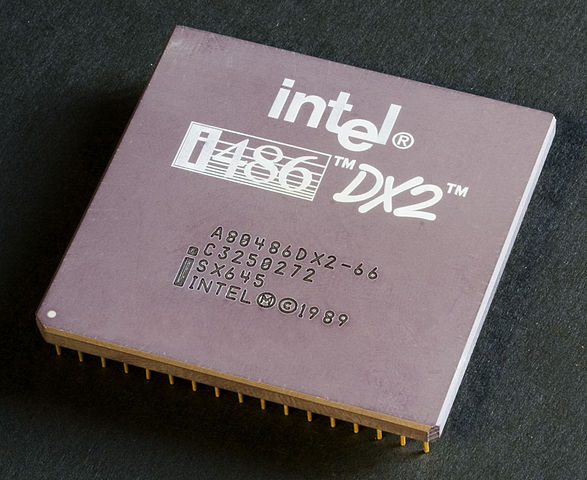
\includegraphics[height=11em]{figs/CPU.jpg}
\hspace{2em}
%https://commons.wikimedia.org/wiki/File:Memory_module_DDRAM_20-03-2006.jpg
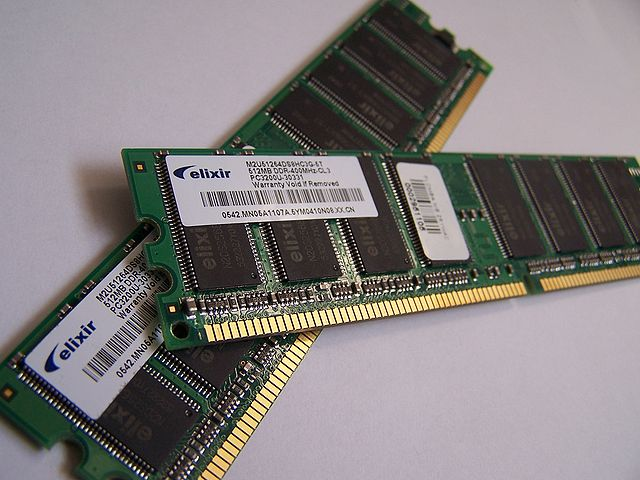
\includegraphics[height=11em]{figs/RAM.jpg}
\caption{Example processor and memory hardware.}
\label{fig.cpuram}
\end{center}
\end{figure}

In 2018 it's common, even for a smartphone, to have four processors and four gigabytes (four billion cells) of memory.
Users generally see and interact with touchscreens, keyboards, and monitors, but it's the processors and memory that perform the actual computations.

When Netflix rents computers from Amazon.com to offer streaming video, what Amazon actually provides is access to server machines that have processors and memory, but no screens or keyboards.

Processors and memory is where computing happens, but they are useless without input/ouput (I/O) devices to receive and send data.
Keyboards and screens are I/O devices, as are the Wifi radios embedded in laptops and smartphones.
Servers like Amazon's have one main I/O device: a network interface which ultimately connects to the laptop where you watch movies.
The Go language was designed primarily to program network connected servers.


\section{What is programming?}

\index{program}

A {\bf program} is a sequence of instructions that specifies how to perform a computation on computer hardware.
The computation might be something mathematical, like solving a system of equations or finding the roots of a polynomial.
It could also be a symbolic computation, like searching and replacing text in a document or (strangely enough) compiling a program.

The details look different in different languages, but a few basic instructions appear in just about every language:

\begin{description}
\item[input:] Get data from the keyboard, a file, the network, a camera, or some other device like a temperature sensor.
\item[output:] Display data on the screen, write it to a file, send it over the network, or activate a device like a door lock.
\item[math:] Perform basic mathematical operations like addition and division.
\item[decisions:] Check for certain conditions and execute the appropriate code.
\item[repetition:] Perform some action repeatedly, usually with some variation.
\end{description}

\index{programming}

Believe it or not, that's pretty much all there is to it.
Every program you've ever used, no matter how complicated, is made up of small instructions that look much like these.
So you can think of {\bf programming} as the process of breaking down a large, complex task into smaller and smaller subtasks.
The process continues until the subtasks are simple enough to be performed with the electronic circuits provided by the hardware.

\section{The hello world program}
\label{hello}

Traditionally, the first program you write when learning a new programming language is called the hello world program.
All it does is display the words ``Hello, World!''\ on the terminal.
In Go, it looks like this:

\index{hello.go}

\begin{lstlisting}
package main

import "fmt"

func main() {
	// display traditional greeting
	fmt.Println("Hello, World!") 
}
\end{lstlisting}

When this program runs it displays:

\begin{stdout}
Hello, World!
\end{stdout}

Notice that the output does not include the quotation marks.


\index{function}
\index{Println function}

Go programs are made up of {\em function} definitions, and functions are made up of {\em statements}.
A {\bf statement} is a line of code that performs a basic action.
The usual way of performing actions is by calling functions that are written by others, such as the Go authors.
So you write functions and your functions, in turn, call other functions.
In the hello world program, this statement calls the {\bf Println} function to display a message on the screen:

\begin{lstlisting}
	fmt.Println("Hello, World!")
\end{lstlisting}

\index{Println}

\java{fmt.Println} displays results on the screen; the name \java{Println} stands for ``print line''.
Confusingly, {\em print} can mean both ``display on the screen'' and ``send to the printer''.
In this book, we'll try to say ``display'' when we mean output to the screen.

\index{case-sensitive}

Go is ``case-sensitive'', which means that uppercase and lowercase are not the same.
In this example, \java{Println} has to begin with an uppercase letter; \java{println} and \java{PRINTLN} won't work.

\index{main function}

A {\bf function} is a sequence of statements.
Functions usually have names, but Go also allows anonymous functions, as we'll see in Chapter XXX.
This code defines a function named \java{main}:

\begin{lstlisting}
func main() {
	// display traditional greeting
	fmt.Println("Hello, World!")
}
\end{lstlisting}

\index{main}

The function name \java{main} is special: when the program runs,
it starts at the first statement in \java{main} and ends when it finishes the last statement.
Later, we will see programs that define more than one function.

\index{\{\} curly braces}
\index{brackets!curly}

Go uses curly braces (\{ and \}) to group things together.
In {\tt hello.go}, the braces contain the body of the function definition.

\index{comment!end-of-line}
\index{statement!comment}

The line that begins with two slashes (\java{//}) is a {\bf comment}, which is a bit of English text that explains the code.
When Go sees \java{//}, it ignores everything from there until the end of the line.
Comments have no effect on the execution of the program, but they make it easier for other programmers (and your future self) to understand what you meant to do.


\index{package}

A {\bf package} is a collection of functions.
The {\tt hello.go} program defines a package named \java{main}. That is also a special name, and it is mandatory for stand-alone programs
--- as opposed to packages designed as parts for larger programs. 

\index{import}

The \java{import} statement declares that our program needs to use the \java{fmt} package, which is part of the Go standard library: a colection of packages providing many ready to use functions. The \java{fmt} name comes from ``format''. The \java{fmt} package has several functions for writing and reading formatted text, such as \java{fmt.Println}.


\section{Compiling Go programs}

\index{high-level language}
\index{language!high-level}

The programming language you will learn in this book is Go, which is a {\bf high-level language}.
Other high-level languages you may have heard of include Java, Python, C, C++, PHP, Ruby, and JavaScript.

\index{machine language}
\index{language!high-level}

Before they can run, programs in high-level languages have to be translated into ``machine language'', the low-level instructions that the computer can follow.
This translation takes some time, which is a small disadvantage of high-level languages.
But high-level languages have two major advantages:

\begin{itemize}

\item It is {\em much} easier to program in a high-level language.
Programs take less time to write, they are shorter and easier to read, and they are more likely to be correct.

\index{portable}

\item High-level languages are {\bf portable}, meaning they can run on different kinds of computers with few or no modifications.
Machine language programs can only run on one kind of computer, and have to be rewritten to run on another.

\end{itemize}

\index{interpret}

Two kinds of programs translate high-level languages into low-level languages: interpreters and compilers.
An {\bf interpreter} reads a high-level program and executes it, meaning that it does what the program says.
It processes the program a little at a time, alternately reading lines and performing computations.
Figure~\ref{fig.interpreter} shows the structure of an interpreter.

\begin{figure}[!ht]
\begin{center}
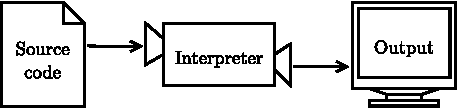
\includegraphics{figs/interpreter.pdf}
\caption{How interpreted languages are executed.}
\label{fig.interpreter}
\end{center}
\end{figure}

\index{compile}
\index{source code}
\index{object code}
\index{executable}

In contrast, a {\bf compiler} reads the entire program and translates it completely before the program starts running.
In this context, the high-level program is called the {\bf source code}, and the translated program is called the {\bf object code} or the {\bf executable}.
Once a program is compiled, you can execute it repeatedly without further translation.
As a result, compiled programs often run faster than interpreted programs.

Figure~\ref{fig.compiler} shows the steps of the development process.
We use the command {\tt go build} to run the Go compile.
It translates {\tt .go} files into binary executable files that store the resulting machine code.
To run the executable, we just call it by name on the command line.

\begin{figure}[!ht]
\begin{center}
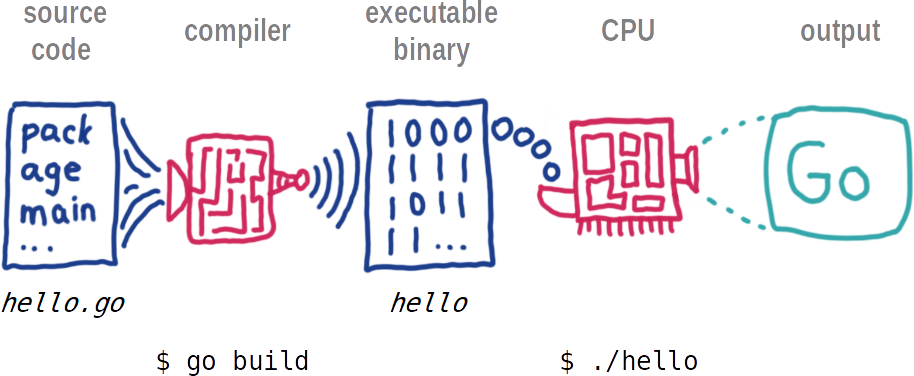
\includegraphics{figs/compiler.png}
\caption{The process of compiling and running a Go program.}
\label{fig.compiler}
\end{center}
\end{figure}

The programmer writes source code in the file {\tt hello.go} and uses {\tt go build} to compile it.
If there are no errors, the compiler saves the executable in the file {\tt hello} (or {\tt hello.exe}, in Windows).
To run the program, the user simply invokes it in the terminal.
The output of the program is then displayed on the screen.

This is how running {\tt hello.go} looks like on the {\tt bash} shell installed by default on GNU/Linux and Mac OS X machines:

\begin{verbatim}
$ ./hello 
Hello, World!
\end{verbatim}

On the Windows command prompt, it's very similar:

\begin{verbatim}
> hello.exe 
Hello, World!
\end{verbatim}


Although it might seem complicated, these steps are automated for you in most program development environments.
Usually you only have to press a button or type a single command to compile and run your program.
On the other hand, it is important to know what steps are happening in the background,
so if something goes wrong you can figure out what it is.


\section{Displaying two messages}

You can put as many statements as you like in the \java{main} method.
For example, to display more than one line of output:

\begin{lstlisting}
package main

import "fmt"

func main() {
	// display traditional greeting
	fmt.Println("Hello, World!") // first line
	fmt.Println("How are you?")  // another line
}
\end{lstlisting}

As this example shows, you can put comments at the end of a line as well as on lines all by themselves.

\index{quote mark}
\index{string}
\index{type!String}
\index{char}

Phrases that appear in quotation marks are called {\bf strings}, because they contain a sequence of characters strung together in memory.
Characters can be letters, ideograms, numbers, punctuation, symbols, spaces, tabs, emojis, etc.

\index{newline}
\index{Println}

\java{fmt.Println} appends a special character, called a {\bf newline}, that breaks the current line and starts a new one.
If you don't want a newline at the end, you can use \java{fmt.Print} instead of \java{fmt.Print}:

\begin{lstlisting}
package main

import "fmt"

func main() {
	fmt.Print("Goodbye, ")
	fmt.Println("cruel world")
}
\end{lstlisting}

\label{goodbye}

In this example, the first statement does not add a newline, so the output appears on a single line as {\tt Goodbye, cruel world}.
Notice that there is a space at the end of the first string, which appears in the output just before the word cruel.


\section{Formatting source code}
\label{formatting}

In Go source code, some spaces are required.
For example, you need at least one space between words, so this program is not legal:

\begin{verbatim}
packagemain

import"fmt"

funcmain() {
	fmt.Println("Hello, World!") 
}
\end{verbatim}


But most other spaces are optional.
For example, this program {\em is} legal:

\begin{lstlisting}
package main
import "fmt"
func main() {
fmt.Println("Hello, World!") 
}
\end{lstlisting}

However, it's harder to read because the structure of the program is not clear.
Tabs and spaces are important for organizing your program visually, making it easier to understand the program and find errors when they occur.

Go also provides a tool, {\tt gofmt}, which rewrites source code in a standard, readable format. Many editors will automatically run {\tt gofmt} when you save a Go source file. 
% LR: similar for VS Code... For example, in DrJava (see Appendix~\ref{drjava}) you can indent your code by selecting all text ({\sf Ctrl+A}) and pressing the {\sf Tab} key.


\section{Escape sequences}

It's possible to display multiple lines of output with only one line of code.
You just have to tell Go where to put the line breaks.

\begin{lstlisting}
package main

import "fmt"

func main() {
	// display traditional greeting
	fmt.Println("Hello!\nHow are you?")
}
\end{lstlisting}

The output is two lines, each ending with a newline character:

\begin{stdout}
Hello!
How are you doing?
\end{stdout}

\index{escape sequence}

The \verb"\n" is an {\bf escape sequence}, or two characters of source code that represent a single character.
(The backslash allows you to ``escape'' the string to write special characters.)
Notice there is no space between \verb"\n" and \verb"How".
If you add a space there, there will be a space at the beginning of the second line.

\begin{table}[!ht]
\begin{center}
\begin{tabular}{|c|c|}
\hline
\verb"\n" & newline \\
\hline
\verb"\t" & tab \\
\hline
\verb'\"' & double quote \\
\hline
\verb"\\" & backslash \\
\hline
\end{tabular}
\caption{Common escape sequences}
\label{tab:escape}
\end{center}
\end{table}

Go has a total of ten escape sequences, and the four most commonly used ones are listed in Table~\ref{tab:escape}.
For example, to write quotation marks inside of strings, you need to escape them with a backslash.

\begin{code}
fmt.Println("She said \"Hello!\" to me.");
\end{code}

The result is:

\begin{stdout}
She said "Hello!" to me.
\end{stdout}

% LR: 2018-01-10: insert ThPy2e "Formal and natural languages" section here
% Drop next section?

\section{What is computer science?}

This book intentionally omits some details about the Go language (such as the other escape sequences),
because our main goal is learning how to think like a computer scientist.
Being able to understand computation is much more valuable than just learning how to write code.

If you're interested in learning more about Go itself, visit the official website: \url{https://golang.org/}.
The interactive tutorial \href{https://tour.golang.org/welcome/1}{\bf A Tour of Go} is a good place to start.

One of the most interesting aspects of writing programs is deciding how to solve a particular problem, especially when there are multiple solutions.
For example, there are numerous ways to sort a list of numbers, and each way has its advantages.
\href{https://www.toptal.com/developers/sorting-algorithms/}{\tt Sorting-algorithms.com} provides animations and descriptions for eight of the most common ways.
In order to determine which way is best for a given situation, we need techniques for describing and analyzing solutions formally.

\index{algorithm}
\index{computer science}

An {\bf algorithm} is a sequence of steps that specifies how to solve a problem.
Some algorithms are faster than others, and some use less space in computer memory.
{\bf Computer science} is the science of algorithms, including their discovery and analysis.
As you learn to develop algorithms for problems you haven't solved before, you will learn to think like a computer scientist.
%It's much more fun to discover new algorithms than to write the code for solutions that other people came up with!

\index{bug}
\index{debugging}

Designing algorithms and writing code is difficult and error-prone.
For historical reasons, programming errors are called {\bf bugs}, and the process of tracking them down and correcting them is called {\bf debugging}.
As you learn to debug your programs, you will develop new problem-solving skills.
You will need to think creatively when unexpected errors happen.

Although it can be frustrating, debugging is an intellectually rich, challenging, and interesting part of computer science.
In some ways, debugging is like detective work.
You are confronted with clues, and you have to infer the processes and events that led to the results you see.
Thinking about how to correct programs and improve their performance sometimes even leads to the discovery of new algorithms.


\section{Debugging programs}
\label{sec:examples}

It is a good idea to read this book in front of a computer so you can try out the examples as you go.
You can run many of the examples directly in DrJava's Interactions Pane (see Appendix~\ref{interactions}).
But if you put the code in a source file, it will be easier to try out variations.

\index{error!message}

Whenever you are experimenting with a new feature, you should also try to make mistakes.
For example, in the hello world program, what happens if you leave out one of the quotation marks?
What if you leave out both?
What if you spell \java{println} wrong?
These kinds of experiments help you remember what you read.
They also help with debugging, because you learn what the error messages mean.
It is better to make mistakes now and on purpose than later on and accidentally.

\index{experimental debugging}
\index{debugging!experimental}

%\index{Holmes, Sherlock}
%\index{Doyle, Arthur Conan}

Debugging is like an experimental science: once you have an idea about what is going wrong, you modify your program and try again.
If your hypothesis was correct, then you can predict the result of the modification, and you take a step closer to a working program.
If your hypothesis was wrong, you have to come up with a new one.
%As Sherlock Holmes pointed out, ``When you have eliminated the impossible, whatever remains, however improbable, must be the truth.''
%(A.~Conan Doyle, {\em The Sign of Four}.)

Programming and debugging should go hand in hand.
Don't just write a bunch of code and then perform trial and error debugging until it all works.
Instead, start with a program that does {\em something} and make small modifications, debugging them as you go, until the program does what you want.
That way you will always have a working program, and it will be easier to isolate errors.

\index{Linux}
\index{Torvalds, Linus}
\index{Greenfield, Larry}

A great example of this principle is the Linux operating system, which contains millions of lines of code.
It started out as a simple program Linus Torvalds used to explore the Intel 80386 chip.
According to Larry Greenfield in {\it The Linux Users' Guide}, ``One of Linus's earlier projects was a program that would switch between printing AAAA and BBBB.
This later evolved to Linux.''

%Later chapters will make more suggestions about debugging and other programming practices.

Finally, programming sometimes brings out strong emotions.
If you are struggling with a difficult bug, you might feel angry, despondent, or embarrassed.
Remember that you are not alone, and virtually every programmer has had similar experiences.
Don't hesitate to reach out to a friend and ask questions!

%That's why this chapter is called, ``The way of the program''.


\section{Vocabulary}

Throughout the book, we try to define each term the first time we use it.
At the end of each chapter, we include the new terms and their definitions in order of appearance.
If you spend some time learning this vocabulary, you will have an easier time reading the following chapters.

\begin{description}

\term{problem solving}
The process of formulating a problem, finding a solution, and expressing the solution.

\term{hardware}
The electronic and mechanical components of a computer, such as CPUs, RAM, and hard disks.

\term{processor}
A computer chip that performs simple instructions like basic arithmetic and logic.

\term{memory}
Circuits that store data as long as the computer is turn on.
Not to be confused with permanent storage devices like hard disks and flash.

\term{program}
A sequence of instructions that specifies how to perform tasks on a computer.
Also known as software.

\term{programming}
The application of problem solving to creating executable computer programs.

\term{statement}
Part of a program that specifies one step of an algorithm.

\term{print statement}
A statement that causes output to be displayed on the screen.

\term{method}
A named sequence of statements.

\term{class}
For now, a collection of related methods.
(We will see later that there is a lot more to it.)

\term{comment}
A part of a program that contains information about the program but has no effect when the program runs.

\term{high-level language}
A programming language that is designed to be easy for humans to read and write.

\term{low-level language}
A programming language that is designed to be easy for a computer to run.
Also called ``machine language'' or ``assembly language''.

\term{portable}
The ability of a program to run on more than one kind of computer.

\term{interpret}
To run a program in a high-level language by translating it one line at a time and immediately executing the corresponding instructions.

\term{compile}
To translate a program in a high-level language into a low-level language, all at once, in preparation for later execution.

\term{source code}
A program in a high-level language, before being compiled.

\term{object code}
The output of the compiler, after translating the program.

\term{executable}
Another name for object code that is ready to run on specific hardware.

\term{byte code}
A special kind of object code used for Java programs.
Byte code is similar to a low-level language, but it is portable like a high-level language.

\term{string}
A sequence of characters; the primary data type for text.

\term{newline}
A special character signifying the end of a line of text.
Also known as line ending, end of line (EOL), or line break.

%\term{whitespace}
%Newlines, tab characters, and other spaces in a source program.
%Whitespace characters are used to separate words, but other than that, they don't affect the behavior of the program.

\term{escape sequence}
A sequence of code that represents a special character when used inside a string.

\term{algorithm}
A procedure or formula for solving a problem, with or without a computer.

\term{computer science}
The scientific and practical approach to computation and its applications.

\term{bug}
An error in a program.

\term{debugging}
The process of finding and removing errors.

\end{description}


\section{Exercises}

At the end of each chapter, we include exercises you can do with the things you've learned.
We encourage you to at least attempt every problem.
You can't learn to program only by reading about it; you have to practice.

Before you can compile and run Java programs, you might have to download and install a few tools.
There are many good options, but we recommend DrJava, which is an ``integrated development environment'' (IDE) well suited for beginners.
Instructions for getting started are in Appendix~\ref{tools}.

The code for this chapter is in the {\tt ch01} directory of {\tt ThinkJavaCode2}.
See page~\pageref{code} for instructions on how to download the repository.
Before you start the exercises, we recommend that you compile and run the examples.


\begin{exercise}  %%V6 Ex1.1

Computer scientists have the annoying habit of using common English words to mean something other than their common English meaning.
For example, in English, statements and comments are the same thing, but in programs they are different.

\begin{enumerate}
\item In computer jargon, what's the difference between a statement and a comment?
\item What does it mean to say that a program is portable?
\item In common English, what does the word compile mean?
\item What is an executable? Why is that word used as a noun?
\end{enumerate}

The glossary at the end of each chapter is intended to highlight words and phrases that have special meanings in computer science.
When you see familiar words, don't assume that you know what they mean!

\end{exercise}


\begin{exercise}  %%V6 Ex1.2

Before you do anything else, find out how to compile and run a Java program.
Some environments provide sample programs similar to the example in Section~\ref{hello}.

\begin{enumerate}
\item Type in the hello world program, then compile and run it.

\item Add a print statement that displays a second message after the ``Hello, World!''.
Say something witty like, ``How are you?''
Compile and run the program again.

\item Add a comment to the program (anywhere), recompile, and run it again.
The new comment should not affect the result.
\end{enumerate}

This exercise may seem trivial, but it is the starting place for many of the programs we will work with.
To debug with confidence, you will need to have confidence in your programming environment.

In some environments, it is easy to lose track of which program is executing.
You might find yourself trying to debug one program while you are accidentally running another.
Adding (and changing) print statements is a simple way to be sure that the program you are looking at is the program you are running.

\end{exercise}


\begin{exercise}  %%V6 Ex1.3

It is a good idea to commit as many errors as you can think of, so that you see what error messages the compiler produces.
Sometimes the compiler tells you exactly what is wrong, and all you have to do is fix it.
But sometimes the error messages are misleading.
Over time you will develop a sense for when you can trust the compiler and when you have to figure things out yourself.

Starting with the hello world program, try out each of the following errors.
After you make each change, compile the program, read the error message (if there is one), and then fix the error.

\begin{enumerate}
\item Remove one of the open curly braces.
\item Remove one of the close curly braces.
\item Instead of \java{main}, write \java{mian}.
\item Remove the word \java{static}.
\item Remove the word \java{public}.
\item Remove the word \java{System}.
\item Replace \java{println} with \java{Println}.
\item Replace \java{println} with \java{print}.
\item Delete one of the parentheses.
\item Add an extra parenthesis.
\end{enumerate}

\end{exercise}


\appendix


\chapter{Debugging}
\index{debugging}

When you are debugging, you should distinguish among different
kinds of errors in order to track them down more quickly:

\begin{itemize}

\item Syntax errors are discovered by the interpreter when it is
  translating the source code into byte code.  They indicate
  that there is something wrong with the structure of the program.
  Example: Omitting the colon at the end of a {\tt def} statement
  generates the somewhat redundant message {\tt SyntaxError: invalid
    syntax}.
\index{syntax error}
\index{error!syntax}

\item Runtime errors are produced by the interpreter if something goes
  wrong while the program is running.  Most runtime error messages
  include information about where the error occurred and what
  functions were executing.  Example: An infinite recursion eventually
  causes the runtime error ``maximum recursion depth exceeded''.
\index{runtime error}
\index{error!runtime}
\index{exception}

\item Semantic errors are problems with a program that runs without
  producing error messages but doesn't do the right thing.  Example:
  An expression may not be evaluated in the order you expect, yielding
  an incorrect result.
\index{semantic error}
\index{error!semantic}

\end{itemize}

The first step in debugging is to figure out which kind of
error you are dealing with.  Although the following sections are
organized by error type, some techniques are
applicable in more than one situation.


\section{Syntax errors}
\index{error message}

Syntax errors are usually easy to fix once you figure out what they
are.  Unfortunately, the error messages are often not helpful.
The most common messages are {\tt SyntaxError: invalid syntax} and
{\tt SyntaxError: invalid token}, neither of which is very informative.

On the other hand, the message does tell you where in the program the
problem occurred.  Actually, it tells you where Python
noticed a problem, which is not necessarily where the error
is.  Sometimes the error is prior to the location of the error
message, often on the preceding line.
\index{incremental development}
\index{development plan!incremental}

If you are building the program incrementally, you should have
a good idea about where the error is.  It will be in the last
line you added.

If you are copying code from a book, start by comparing
your code to the book's code very carefully.  Check every character.
At the same time, remember that the book might be wrong, so
if you see something that looks like a syntax error, it might be.

Here are some ways to avoid the most common syntax errors:
\index{syntax}

\begin{enumerate}

\item Make sure you are not using a Python keyword for a variable name.
\index{keyword}

\item Check that you have a colon at the end of the header of every
compound statement, including {\tt for}, {\tt while},
{\tt if}, and {\tt def} statements.
\index{header}
\index{colon}

\item Make sure that any strings in the code have matching
quotation marks.  Make sure that all quotation marks are
``straight quotes'', not ``curly quotes''.
\index{quotation mark}

\item If you have multiline strings with triple quotes (single or double), make
sure you have terminated the string properly.  An unterminated string
may cause an {\tt invalid token} error at the end of your program,
or it may treat the following part of the program as a string until it
comes to the next string.  In the second case, it might not produce an error
message at all!
\index{multiline string}
\index{string!multiline}

\item An unclosed opening operator---\verb+(+, \verb+{+, or
  \verb+[+---makes Python continue with the next line as part of the
  current statement.  Generally, an error occurs almost immediately in
  the next line.

\item Check for the classic {\tt =} instead of {\tt ==} inside
a conditional.
\index{conditional}

\item Check the indentation to make sure it lines up the way it
is supposed to.  Python can handle space and tabs, but if you mix
them it can cause problems.  The best way to avoid this problem
is to use a text editor that knows about Python and generates
consistent indentation.
\index{indentation}
\index{whitespace}

\item If you have non-ASCII characters in the code (including strings
and comments), that might cause a problem, although Python 3 usually
handles non-ASCII characters.  Be careful if you paste in text from
a web page or other source.

\end{enumerate}

If nothing works, move on to the next section...


\subsection{I keep making changes and it makes no difference.}

If the interpreter says there is an error and you don't see it, that
might be because you and the interpreter are not looking at the same
code.  Check your programming environment to make sure that the
program you are editing is the one Python is trying to run.

If you are not sure, try putting an obvious and deliberate syntax
error at the beginning of the program.  Now run it again.  If the
interpreter doesn't find the new error, you are not running the
new code.

There are a few likely culprits:

\begin{itemize}

\item You edited the file and forgot to save the changes before
running it again.  Some programming environments do this
for you, but some don't.

\item You changed the name of the file, but you are still running
the old name.

\item Something in your development environment is configured
incorrectly.

\item If you are writing a module and using {\tt import},
make sure you don't give your module the same name as one
of the standard Python modules.

\item If you are using {\tt import} to read a module, remember
that you have to restart the interpreter or use {\tt reload}
to read a modified file.  If you import the module again, it
doesn't do anything.
\index{module!reload}
\index{reload function}
\index{function!reload}

\end{itemize}

If you get stuck and you can't figure out what is going on, one
approach is to start again with a new program like ``Hello, World!'',
and make sure you can get a known program to run.  Then gradually add
the pieces of the original program to the new one.


\section{Runtime errors}

Once your program is syntactically correct,
Python can read it and at least start running it.  What could
possibly go wrong?


\subsection{My program does absolutely nothing.}

This problem is most common when your file consists of functions and
classes but does not actually invoke a function to start execution.
This may be intentional if you only plan to import this module to
supply classes and functions.

If it is not intentional, make sure there is a function call
in the program, and make sure the flow of execution reaches
it (see ``Flow of Execution'' below).


\subsection{My program hangs.}
\index{infinite loop}
\index{infinite recursion}
\index{hanging}

If a program stops and seems to be doing nothing, it is ``hanging''.
Often that means that it is caught in an infinite loop or infinite
recursion.

\begin{itemize}

\item If there is a particular loop that you suspect is the
problem, add a {\tt print} statement immediately before the loop that says
``entering the loop'' and another immediately after that says
``exiting the loop''.

Run the program.  If you get the first message and not the second,
you've got an infinite loop.  Go to the ``Infinite Loop'' section
below.

\item Most of the time, an infinite recursion will cause the program
to run for a while and then produce a ``RuntimeError: Maximum
recursion depth exceeded'' error.  If that happens, go to the
``Infinite Recursion'' section below.

If you are not getting this error but you suspect there is a problem
with a recursive method or function, you can still use the techniques
in the ``Infinite Recursion'' section.

\item If neither of those steps works, start testing other
loops and other recursive functions and methods.

\item If that doesn't work, then it is possible that
you don't understand the flow of execution in your program.
Go to the ``Flow of Execution'' section below.

\end{itemize}


\subsubsection{Infinite Loop}
\index{infinite loop}
\index{loop!infinite}
\index{condition}
\index{loop!condition}

If you think you have an infinite loop and you think you know
what loop is causing the problem, add a {\tt print} statement at
the end of the loop that prints the values of the variables in
the condition and the value of the condition.

For example:

\begin{verbatim}
while x > 0 and y < 0 :
    # do something to x
    # do something to y

    print('x: ', x)
    print('y: ', y)
    print("condition: ", (x > 0 and y < 0))
\end{verbatim}
%
Now when you run the program, you will see three lines of output
for each time through the loop.  The last time through the
loop, the condition should be {\tt False}.  If the loop keeps
going, you will be able to see the values of {\tt x} and {\tt y},
and you might figure out why they are not being updated correctly.


\subsubsection{Infinite Recursion}
\index{infinite recursion}
\index{recursion!infinite}

Most of the time, infinite recursion causes the program to run
for a while and then produce a {\tt Maximum recursion depth exceeded}
error.

If you suspect that a function is causing an infinite
recursion, make sure that there is a base case.
There should be some condition that causes the
function to return without making a recursive invocation.
If not, you need to rethink the algorithm and identify a base
case.

If there is a base case but the program doesn't seem to be reaching
it, add a {\tt print} statement at the beginning of the function
that prints the parameters.  Now when you run the program, you will see
a few lines of output every time the function is invoked,
and you will see the parameter values.  If the parameters are not moving
toward the base case, you will get some ideas about why not.


\subsubsection{Flow of Execution}
\index{flow of execution}

If you are not sure how the flow of execution is moving through
your program, add {\tt print} statements to the beginning of each
function with a message like ``entering function {\tt foo}'', where
{\tt foo} is the name of the function.

Now when you run the program, it will print a trace of each
function as it is invoked.


\subsection{When I run the program I get an exception.}
\index{exception}
\index{runtime error}

If something goes wrong during runtime, Python
prints a message that includes the name of the
exception, the line of the program where the problem occurred,
and a traceback.
\index{traceback}

The traceback identifies the function that is currently running, and
then the function that called it, and then the function that called
{\em that}, and so on.  In other words, it traces the sequence of
function calls that got you to where you are, including the line
number in your file where each call occurred.

The first step is to examine the place in the program where
the error occurred and see if you can figure out what happened.
These are some of the most common runtime errors:

\begin{description}

\item[NameError:]  You are trying to use a variable that doesn't
exist in the current environment.  Check if the name
is spelled right, or at least consistently.
And remember that local variables are local; you
cannot refer to them from outside the function where they are defined.
\index{NameError}
\index{exception!NameError}

\item[TypeError:] There are several possible causes:
\index{TypeError}
\index{exception!TypeError}

\begin{itemize}

\item  You are trying to use a value improperly.  Example: indexing
a string, list, or tuple with something other than an integer.
\index{index}

\item There is a mismatch between the items in a format string and
the items passed for conversion.  This can happen if either the number
of items does not match or an invalid conversion is called for.
\index{format operator}
\index{operator!format}

\item You are passing the wrong number of arguments to a function.
For methods, look at the method definition and
check that the first parameter is {\tt self}.  Then look at the
method invocation; make sure you are invoking the method on an
object with the right type and providing the other arguments
correctly.

\end{itemize}

\item[KeyError:]  You are trying to access an element of a dictionary
using a key that the dictionary does not contain.  If the keys
are strings, remember that capitalization matters.
\index{KeyError}
\index{exception!KeyError}
\index{dictionary}

\item[AttributeError:] You are trying to access an attribute or method
  that does not exist.  Check the spelling!  You can use the built-in
  function {\tt vars} to list the attributes that do exist.
\index{dir function}
\index{function!dir}

If an AttributeError indicates that an object has {\tt NoneType},
that means that it is {\tt None}.  So the problem is not the
attribute name, but the object.

The reason the object is none might be that you forgot
to return a value from a function; if you get to the end of
a function without hitting a {\tt return} statement, it returns
{\tt None}.  Another common cause is using the result from
a list method, like {\tt sort}, that returns {\tt None}.
\index{AttributeError}
\index{exception!AttributeError}

\item[IndexError:] The index you are using
to access a list, string, or tuple is greater than
its length minus one.  Immediately before the site of the error,
add a {\tt print} statement to display
the value of the index and the length of the array.
Is the array the right size?  Is the index the right value?
\index{IndexError}
\index{exception!IndexError}

\end{description}

The Python debugger ({\tt pdb}) is useful for tracking down
exceptions because it allows you to examine the state of the
program immediately before the error.  You can read
about {\tt pdb} at \url{https://docs.python.org/3/library/pdb.html}.
\index{debugger (pdb)}
\index{pdb (Python debugger)}


\subsection{I added so many {\tt print} statements I get inundated with
output.}
\index{print statement}
\index{statement!print}

One of the problems with using {\tt print} statements for debugging
is that you can end up buried in output.  There are two ways
to proceed: simplify the output or simplify the program.

To simplify the output, you can remove or comment out {\tt print}
statements that aren't helping, or combine them, or format
the output so it is easier to understand.

To simplify the program, there are several things you can do.  First,
scale down the problem the program is working on.  For example, if you
are searching a list, search a {\em small} list.  If the program takes
input from the user, give it the simplest input that causes the
problem.
\index{dead code}

Second, clean up the program.  Remove dead code and reorganize the
program to make it as easy to read as possible.  For example, if you
suspect that the problem is in a deeply nested part of the program,
try rewriting that part with simpler structure.  If you suspect a
large function, try splitting it into smaller functions and testing them
separately.
\index{testing!minimal test case}
\index{test case, minimal}

Often the process of finding the minimal test case leads you to the
bug.  If you find that a program works in one situation but not in
another, that gives you a clue about what is going on.

Similarly, rewriting a piece of code can help you find subtle
bugs.  If you make a change that you think shouldn't affect the
program, and it does, that can tip you off.


\section{Semantic errors}

In some ways, semantic errors are the hardest to debug,
because the interpreter provides no information
about what is wrong.  Only you know what the program is supposed to
do.
\index{semantic error}
\index{error!semantic}

The first step is to make a connection between the program
text and the behavior you are seeing.  You need a hypothesis
about what the program is actually doing.  One of the things
that makes that hard is that computers run so fast.

You will often wish that you could slow the program down to human
speed, and with some debuggers you can.  But the time it takes to
insert a few well-placed {\tt print} statements is often short compared to
setting up the debugger, inserting and removing breakpoints, and
``stepping'' the program to where the error is occurring.


\subsection{My program doesn't work.}

You should ask yourself these questions:

\begin{itemize}

\item Is there something the program was supposed to do but
which doesn't seem to be happening?  Find the section of the code
that performs that function and make sure it is executing when
you think it should.

\item Is something happening that shouldn't?  Find code in
your program that performs that function and see if it is
executing when it shouldn't.

\item Is a section of code producing an effect that is not
what you expected?  Make sure that you understand the code in
question, especially if it involves functions or methods in
other Python modules.  Read the documentation for the functions you call.
Try them out by writing simple test cases and checking the results.

\end{itemize}

In order to program, you need a mental model of how
programs work.  If you write a program that doesn't do what you expect,
often the problem is not in the program; it's in your mental
model.
\index{model, mental}
\index{mental model}

The best way to correct your mental model is to break the program
into its components (usually the functions and methods) and test
each component independently.  Once you find the discrepancy
between your model and reality, you can solve the problem.

Of course, you should be building and testing components as you
develop the program.  If you encounter a problem,
there should be only a small amount of new code
that is not known to be correct.


\subsection{I've got a big hairy expression and it doesn't
do what I expect.}
\index{expression!big and hairy}
\index{big, hairy expression}

Writing complex expressions is fine as long as they are readable,
but they can be hard to debug.  It is often a good idea to
break a complex expression into a series of assignments to
temporary variables.

For example:

\begin{verbatim}
self.hands[i].addCard(self.hands[self.findNeighbor(i)].popCard())
\end{verbatim}
%
This can be rewritten as:

\begin{verbatim}
neighbor = self.findNeighbor(i)
pickedCard = self.hands[neighbor].popCard()
self.hands[i].addCard(pickedCard)
\end{verbatim}
%
The explicit version is easier to read because the variable
names provide additional documentation, and it is easier to debug
because you can check the types of the intermediate variables
and display their values.
\index{temporary variable}
\index{variable!temporary}

Another problem that can occur with big expressions is
that the order of evaluation may not be what you expect.
For example, if you are translating the expression
$\frac{x}{2 \pi}$ into Python, you might write:

\begin{verbatim}
y = x / 2 * math.pi
\end{verbatim}
%
That is not correct because multiplication and division have
the same precedence and are evaluated from left to right.
So this expression computes $x \pi / 2$.
\index{order of operations}
\index{precedence}

A good way to debug expressions is to add parentheses to make
the order of evaluation explicit:

\begin{verbatim}
 y = x / (2 * math.pi)
\end{verbatim}
%
Whenever you are not sure of the order of evaluation, use
parentheses.  Not only will the program be correct (in the sense
of doing what you intended), it will also be more readable for
other people who haven't memorized the order of operations.


\subsection{I've got a function that doesn't return what I
expect.}
\index{return statement}
\index{statement!return}

If you have a {\tt return} statement with a complex expression,
you don't have a chance to print the result before
returning.  Again, you can use a temporary variable.  For
example, instead of:

\begin{verbatim}
return self.hands[i].removeMatches()
\end{verbatim}
%
you could write:

\begin{verbatim}
count = self.hands[i].removeMatches()
return count
\end{verbatim}
%
Now you have the opportunity to display the value of
{\tt count} before returning.


\subsection{I'm really, really stuck and I need help.}

First, try getting away from the computer for a few minutes.
Computers emit waves that affect the brain, causing these
symptoms:

\begin{itemize}

\item Frustration and rage.
\index{frustration}
\index{rage}
\index{debugging!emotional response}
\index{emotional debugging}

\item Superstitious beliefs (``the computer hates me'') and
magical thinking (``the program only works when I wear my
hat backward'').
\index{debugging!superstition}
\index{superstitious debugging}

\item Random walk programming (the attempt to program by writing
every possible program and choosing the one that does the right
thing).
\index{random walk programming}
\index{development plan!random walk programming}

\end{itemize}

If you find yourself suffering from any of these symptoms, get
up and go for a walk.  When you are calm, think about the program.
What is it doing?  What are some possible causes of that
behavior?  When was the last time you had a working program,
and what did you do next?

Sometimes it just takes time to find a bug.  I often find bugs
when I am away from the computer and let my mind wander.  Some
of the best places to find bugs are trains, showers, and in bed,
just before you fall asleep.


\subsection{No, I really need help.}

It happens.  Even the best programmers occasionally get stuck.
Sometimes you work on a program so long that you can't see the
error.  You need a fresh pair of eyes.

Before you bring someone else in, make sure you are prepared.
Your program should be as simple
as possible, and you should be working on the smallest input
that causes the error.  You should have {\tt print} statements in the
appropriate places (and the output they produce should be
comprehensible).  You should understand the problem well enough
to describe it concisely.

When you bring someone in to help, be sure to give
them the information they need:

\begin{itemize}

\item If there is an error message, what is it
and what part of the program does it indicate?

\item What was the last thing you did before this error occurred?
What were the last lines of code that you wrote, or what is
the new test case that fails?

\item What have you tried so far, and what have you learned?

\end{itemize}

When you find the bug, take a second to think about what you
could have done to find it faster.  Next time you see something
similar, you will be able to find the bug more quickly.

Remember, the goal is not just to make the program
work.  The goal is to learn how to make the program work.


\chapter{Analysis of Algorithms}
\label{algorithms}

\begin{quote}
This appendix is an edited excerpt from {\it Think Complexity}, by
Allen B. Downey, also published by O'Reilly Media (2012).  When you
are done with this book, you might want to move on to that one.
\end{quote}

{\bf Analysis of algorithms} is a branch of computer science that
studies the performance of algorithms, especially their run time and
space requirements.  See
\url{http://en.wikipedia.org/wiki/Analysis_of_algorithms}.
\index{algorithm} \index{analysis of algorithms}

The practical goal of algorithm analysis is to predict the performance
of different algorithms in order to guide design decisions.

During the 2008 United States Presidential Campaign, candidate
Barack Obama was asked to perform an impromptu analysis when
he visited Google.  Chief executive Eric Schmidt jokingly asked him
for ``the most efficient way to sort a million 32-bit integers.''
Obama had apparently been tipped off, because he quickly
replied, ``I think the bubble sort would be the wrong way to go.''
See \url{http://www.youtube.com/watch?v=k4RRi_ntQc8}.
\index{Obama, Barack}
\index{Schmidt, Eric}
\index{bubble sort}

This is true: bubble sort is conceptually simple but slow for
large datasets.  The answer Schmidt was probably looking for is
``radix sort'' (\url{http://en.wikipedia.org/wiki/Radix_sort})\footnote{
But if you get a question like this in an interview, I think
a better answer is, ``The fastest way to sort a million integers
is to use whatever sort function is provided by the language
I'm using.  Its performance is good enough for the vast majority
of applications, but if it turned out that my application was too
slow, I would use a profiler to see where the time was being
spent.  If it looked like a faster sort algorithm would have
a significant effect on performance, then I would look
around for a good implementation of radix sort.''}.
\index{radix sort}

The goal of algorithm analysis is to make meaningful
comparisons between algorithms, but there are some problems:
\index{comparing algorithms}

\begin{itemize}

\item The relative performance of the algorithms might
depend on characteristics of the hardware, so one algorithm
might be faster on Machine A, another on Machine B.
The general solution to this problem is to specify a
{\bf machine model} and analyze the number of steps, or
operations, an algorithm requires under a given model.
\index{machine model}

\item Relative performance might depend on the details of
the dataset.  For example, some sorting
algorithms run faster if the data are already partially sorted;
other algorithms run slower in this case.
A common way to avoid this problem is to analyze the
{\bf worst case} scenario.  It is sometimes useful to
analyze average case performance, but that's usually harder,
and it might not be obvious what set of cases to average over.
\index{worst case}
\index{average case}

\item Relative performance also depends on the size of the
problem.  A sorting algorithm that is fast for small lists
might be slow for long lists.
The usual solution to this problem is to express run time
(or number of operations) as a function of problem size,
and group functions into categories depending on how quickly
they grow as problem size increases.

\end{itemize}

The good thing about this kind of comparison is that it lends
itself to simple classification of algorithms.  For example,
if I know that the run time of Algorithm A tends to be
proportional to the size of the input, $n$, and Algorithm B
tends to be proportional to $n^2$, then I
expect A to be faster than B, at least for large values of $n$.

This kind of analysis comes with some caveats, but we'll get
to that later.


\section{Order of growth}

Suppose you have analyzed two algorithms and expressed
their run times in terms of the size of the input:
Algorithm A takes $100n+1$ steps to solve a problem with
size $n$; Algorithm B takes $n^2 + n + 1$ steps.
\index{order of growth}

The following table shows the run time of these algorithms
for different problem sizes:

\begin{tabular}{|r|r|r|}
\hline
Input     &   Run time of     & Run time of \\
size      &   Algorithm A     & Algorithm B \\
\hline
10        &   1 001           & 111         \\
100       &   10 001          & 10 101         \\
1 000     &   100 001         & 1 001 001         \\
10 000    &   1 000 001       & $> 10^{10}$         \\
\hline
\end{tabular}

At $n=10$, Algorithm A looks pretty bad; it takes almost 10 times
longer than Algorithm B.  But for $n=100$ they are about the same, and
for larger values A is much better.

The fundamental reason is that for large values of $n$, any function
that contains an $n^2$ term will grow faster than a function whose
leading term is $n$.  The {\bf leading term} is the term with the
highest exponent.
\index{leading term}
\index{exponent}

For Algorithm A, the leading term has a large coefficient, 100, which
is why B does better than A for small $n$.  But regardless of the
coefficients, there will always be some value of $n$ where
$a n^2 > b n$, for any values of $a$ and $b$.
\index{leading coefficient}

The same argument applies to the non-leading terms.  Even if the run
time of Algorithm A were $n+1000000$, it would still be better than
Algorithm B for sufficiently large $n$.

In general, we expect an algorithm with a smaller leading term to be a
better algorithm for large problems, but for smaller problems, there
may be a {\bf crossover point} where another algorithm is better.  The
location of the crossover point depends on the details of the
algorithms, the inputs, and the hardware, so it is usually ignored for
purposes of algorithmic analysis.  But that doesn't mean you can forget
about it.
\index{crossover point}

If two algorithms have the same leading order term, it is hard to say
which is better; again, the answer depends on the details.  So for
algorithmic analysis, functions with the same leading term
are considered equivalent, even if they have different coefficients.

An {\bf order of growth} is a set of functions whose growth
behavior is considered equivalent.  For example, $2n$, $100n$ and $n+1$ 
belong to the same order of growth, which is written $O(n)$ in
{\bf Big-Oh notation} and often called {\bf linear} because every function
in the set grows linearly with $n$.
\index{big-oh notation}
\index{linear growth}

All functions with the leading term $n^2$ belong to $O(n^2)$; they are
called {\bf quadratic}.
\index{quadratic growth}

The following table shows some of the orders of growth that
appear most commonly in algorithmic analysis,
in increasing order of badness.
\index{badness}

\begin{tabular}{|r|r|r|}
\hline
Order of     &   Name      \\
growth       &               \\
\hline
$O(1)$             & constant \\
$O(\log_b n)$      & logarithmic (for any $b$) \\
$O(n)$             & linear \\
$O(n \log_b n)$    & linearithmic \\
$O(n^2)$           & quadratic     \\
$O(n^3)$           & cubic     \\
$O(c^n)$           & exponential (for any $c$)    \\
\hline
\end{tabular}

For the logarithmic terms, the base of the logarithm doesn't matter;
changing bases is the equivalent of multiplying by a constant, which
doesn't change the order of growth.  Similarly, all exponential
functions belong to the same order of growth regardless of the base of
the exponent.
Exponential functions grow very quickly, so exponential algorithms are
only useful for small problems.
\index{logarithmic growth}
\index{exponential growth}


\begin{exercise}

Read the Wikipedia page on Big-Oh notation at
\url{http://en.wikipedia.org/wiki/Big_O_notation} and
answer the following questions:

\begin{enumerate}
\item What is the order of growth of $n^3 + n^2$?
What about $1000000 n^3 + n^2$?
What about $n^3 + 1000000 n^2$?

\item What is the order of growth of $(n^2 + n) \cdot (n + 1)$?  Before
  you start multiplying, remember that you only need the leading term.

\item If $f$ is in $O(g)$, for some unspecified function $g$, what can
  we say about $af+b$?

\item If $f_1$ and $f_2$ are in $O(g)$, what can we say about $f_1 + f_2$?

\item If  $f_1$ is in $O(g)$
and $f_2$ is in $O(h)$,
what can we say about  $f_1 + f_2$?

\item If  $f_1$ is in $O(g)$ and $f_2$ is $O(h)$,
what can we say about  $f_1 \cdot f_2$?
\end{enumerate}

\end{exercise}

Programmers who care about performance often find this kind of
analysis hard to swallow.  They have a point: sometimes the
coefficients and the non-leading terms make a real difference.
Sometimes the details of the hardware, the programming language, and
the characteristics of the input make a big difference.  And for small
problems asymptotic behavior is irrelevant.

But if you keep those caveats in mind, algorithmic analysis is a
useful tool.  At least for large problems, the ``better'' algorithm
is usually better, and sometimes it is {\em much} better.  The
difference between two algorithms with the same order of growth is
usually a constant factor, but the difference between a good algorithm
and a bad algorithm is unbounded!


\section{Analysis of basic Python operations}

In Python, most arithmetic operations are constant time;
multiplication usually takes longer than addition and subtraction, and
division takes even longer, but these run times don't depend on the
magnitude of the operands.  Very large integers are an exception; in
that case the run time increases with the number of digits.
\index{analysis of primitives}

Indexing operations---reading or writing elements in a sequence
or dictionary---are also constant time, regardless of the size
of the data structure.
\index{indexing}

A {\tt for} loop that traverses a sequence or dictionary is
usually linear, as long as all of the operations in the body
of the loop are constant time.  For example, adding up the
elements of a list is linear:

\begin{verbatim}
    total = 0
    for x in t:
        total += x
\end{verbatim}

The built-in function {\tt sum} is also linear because it does
the same thing, but it tends to be faster because it is a more
efficient implementation; in the language of algorithmic analysis,
it has a smaller leading coefficient.

As a rule of thumb, if the body of a loop is in $O(n^a)$ then
the whole loop is in $O(n^{a+1})$.  The exception is if you can
show that the loop exits after a constant number of iterations.
If a loop runs $k$ times regardless of $n$, then
the loop is in $O(n^a)$, even for large $k$.

Multiplying by $k$ doesn't change the order of growth, but neither
does dividing.  So if the body of a loop is in $O(n^a)$ and it runs
$n/k$ times, the loop is in $O(n^{a+1})$, even for large $k$.

Most string and tuple operations are linear, except indexing and {\tt
  len}, which are constant time.  The built-in functions {\tt min} and
{\tt max} are linear.  The run-time of a slice operation is
proportional to the length of the output, but independent of the size
of the input.
\index{string methods}
\index{tuple methods}

String concatenation is linear; the run time depends on the sum
of the lengths of the operands.
\index{string concatenation}

All string methods are linear, but if the lengths of
the strings are bounded by a constant---for example, operations on single
characters---they are considered constant time.
The string method {\tt join} is linear; the run time depends on
the total length of the strings.
\index{join@{\tt join}}

Most list methods are linear, but there are some exceptions:
\index{list methods}

\begin{itemize}

\item Adding an element to the end of a list is constant time on
average; when it runs out of room it occasionally gets copied
to a bigger location, but the total time for $n$ operations
is $O(n)$, so the average time for each
operation is $O(1)$.

\item Removing an element from the end of a list is constant time.

\item Sorting is $O(n \log n)$.
\index{sorting}

\end{itemize}

Most dictionary operations and methods are constant time, but
there are some exceptions:
\index{dictionary methods}

\begin{itemize}

\item The run time of {\tt update} is
  proportional to the size of the dictionary passed as a parameter,
  not the dictionary being updated.

\item {\tt keys}, {\tt values} and {\tt items} are constant time because 
  they return iterators.  But
  if you loop through the iterators, the loop will be linear.
\index{iterator}

\end{itemize}

The performance of dictionaries is one of the minor miracles of
computer science.  We will see how they work in
Section~\ref{hashtable}.


\begin{exercise}

Read the Wikipedia page on sorting algorithms at
\url{http://en.wikipedia.org/wiki/Sorting_algorithm} and answer
the following questions:
\index{sorting}

\begin{enumerate}

\item What is a ``comparison sort?'' What is the best worst-case order
  of growth for a comparison sort?  What is the best worst-case order
  of growth for any sort algorithm?
\index{comparison sort}

\item What is the order of growth of bubble sort, and why does Barack
  Obama think it is ``the wrong way to go?''

\item What is the order of growth of radix sort?  What preconditions
  do we need to use it?

\item What is a stable sort and why might it matter in practice?
\index{stable sort}

\item What is the worst sorting algorithm (that has a name)?

\item What sort algorithm does the C library use?  What sort algorithm
  does Python use?  Are these algorithms stable?  You might have to
  Google around to find these answers.

\item Many of the non-comparison sorts are linear, so why does does
  Python use an $O(n \log n)$ comparison sort?

\end{enumerate}

\end{exercise}


\section{Analysis of search algorithms}

A {\bf search} is an algorithm that takes a collection and a target
item and determines whether the target is in the collection, often
returning the index of the target.
\index{search}

The simplest search algorithm is a ``linear search'', which traverses
the items of the collection in order, stopping if it finds the target.
In the worst case it has to traverse the entire collection, so the run
time is linear.
\index{linear search}

The {\tt in} operator for sequences uses a linear search; so do string
methods like {\tt find} and {\tt count}.
\index{in@{\tt in} operator}

If the elements of the sequence are in order, you can use a {\bf
  bisection search}, which is $O(\log n)$.  Bisection search is
similar to the algorithm you might use to look a word up in a
dictionary (a paper dictionary, not the data structure).  Instead of
starting at the beginning and checking each item in order, you start
with the item in the middle and check whether the word you are looking
for comes before or after.  If it comes before, then you search the
first half of the sequence.  Otherwise you search the second half.
Either way, you cut the number of remaining items in half.
\index{bisection search}

If the sequence has 1,000,000 items, it will take about 20 steps to
find the word or conclude that it's not there.  So that's about 50,000
times faster than a linear search.

Bisection search can be much faster than linear search, but
it requires the sequence to be in order, which might require
extra work.

There is another data structure, called a {\bf hashtable} that
is even faster---it can do a search in constant time---and it
doesn't require the items to be sorted.  Python dictionaries
are implemented using hashtables, which is why most dictionary
operations, including the {\tt in} operator, are constant time.


\section{Hashtables}
\label{hashtable}

To explain how hashtables work and why their performance is so
good, I start with a simple implementation of a map and
gradually improve it until it's a hashtable.
\index{hashtable}

I use Python to demonstrate these implementations, but in real
life you wouldn't write code like this in Python; you would just use a
dictionary!  So for the rest of this chapter, you have to imagine that
dictionaries don't exist and you want to implement a data structure
that maps from keys to values.  The operations you have to
implement are:

\begin{description}

\item[{\tt add(k, v)}:] Add a new item that maps from key {\tt k}
to value {\tt v}.  With a Python dictionary, {\tt d}, this operation
is written {\tt d[k] = v}.

\item[{\tt get(k)}:] Look up and return the value that corresponds
to key {\tt k}.  With a Python dictionary, {\tt d}, this operation
is written {\tt d[k]} or {\tt d.get(k)}.

\end{description}

For now, I assume that each key only appears once.
The simplest implementation of this interface uses a list of
tuples, where each tuple is a key-value pair.
\index{LinearMap@{\tt LinearMap}}

\begin{verbatim}
class LinearMap:

    def __init__(self):
        self.items = []

    def add(self, k, v):
        self.items.append((k, v))

    def get(self, k):
        for key, val in self.items:
            if key == k:
                return val
        raise KeyError
\end{verbatim}

{\tt add} appends a key-value tuple to the list of items, which
takes constant time.

{\tt get} uses a {\tt for} loop to search the list:
if it finds the target key it returns the corresponding value;
otherwise it raises a {\tt KeyError}.
So {\tt get} is linear.
\index{KeyError@{\tt KeyError}}

An alternative is to keep the list sorted by key.  Then {\tt get}
could use a bisection search, which is $O(\log n)$.  But inserting a
new item in the middle of a list is linear, so this might not be the
best option.  There are other data structures that can implement {\tt
  add} and {\tt get} in log time, but that's still not as good as
constant time, so let's move on.
\index{red-black tree}

One way to improve {\tt LinearMap} is to break the list of key-value
pairs into smaller lists.  Here's an implementation called
{\tt BetterMap}, which is a list of 100 LinearMaps.  As we'll see
in a second, the order of growth for {\tt get} is still linear,
but {\tt BetterMap} is a step on the path toward hashtables:
\index{BetterMap@{\tt BetterMap}}

\begin{verbatim}
class BetterMap:

    def __init__(self, n=100):
        self.maps = []
        for i in range(n):
            self.maps.append(LinearMap())

    def find_map(self, k):
        index = hash(k) % len(self.maps)
        return self.maps[index]

    def add(self, k, v):
        m = self.find_map(k)
        m.add(k, v)

    def get(self, k):
        m = self.find_map(k)
        return m.get(k)
\end{verbatim}

\verb"__init__" makes a list of {\tt n} {\tt LinearMap}s.

\verb"find_map" is used by
{\tt add} and {\tt get}
to figure out which map to put the
new item in, or which map to search.

\verb"find_map" uses the built-in function {\tt hash}, which takes
almost any Python object and returns an integer.  A limitation of this
implementation is that it only works with hashable keys.  Mutable
types like lists and dictionaries are unhashable.
\index{hash function}

Hashable objects that are considered equivalent return the same hash
value, but the converse is not necessarily true: two objects with
different values can return the same hash value.

\verb"find_map" uses the modulus operator to wrap the hash values
into the range from 0 to {\tt len(self.maps)}, so the result is a legal
index into the list.  Of course, this means that many different
hash values will wrap onto the same index.  But if the hash function
spreads things out pretty evenly (which is what hash functions
are designed to do), then we expect $n/100$ items per LinearMap.

Since the run time of {\tt LinearMap.get} is proportional to the
number of items, we expect BetterMap to be about 100 times faster
than LinearMap.  The order of growth is still linear, but the
leading coefficient is smaller.  That's nice, but still not
as good as a hashtable.

Here (finally) is the crucial idea that makes hashtables fast: if you
can keep the maximum length of the LinearMaps bounded, {\tt
  LinearMap.get} is constant time.  All you have to do is keep track
of the number of items and when the number of
items per LinearMap exceeds a threshold, resize the hashtable by
adding more LinearMaps.
\index{bounded}

Here is an implementation of a hashtable:
\index{HashMap}

\begin{verbatim}
class HashMap:

    def __init__(self):
        self.maps = BetterMap(2)
        self.num = 0

    def get(self, k):
        return self.maps.get(k)

    def add(self, k, v):
        if self.num == len(self.maps.maps):
            self.resize()

        self.maps.add(k, v)
        self.num += 1

    def resize(self):
        new_maps = BetterMap(self.num * 2)

        for m in self.maps.maps:
            for k, v in m.items:
                new_maps.add(k, v)

        self.maps = new_maps
\end{verbatim}

Each {\tt HashMap} contains a {\tt BetterMap}; \verb"__init__" starts
with just 2 LinearMaps and initializes {\tt num}, which keeps track of
the number of items.

{\tt get} just dispatches to {\tt BetterMap}.  The real work happens
in {\tt add}, which checks the number of items and the size of the
{\tt BetterMap}: if they are equal, the average number of items per
LinearMap is 1, so it calls {\tt resize}.

{\tt resize} make a new {\tt BetterMap}, twice as big as the previous
one, and then ``rehashes'' the items from the old map to the new.

Rehashing is necessary because changing the number of LinearMaps
changes the denominator of the modulus operator in
\verb"find_map".  That means that some objects that used
to hash into the same LinearMap will get split up (which is
what we wanted, right?).
\index{rehashing}

Rehashing is linear, so
{\tt resize} is linear, which might seem bad, since I promised
that {\tt add} would be constant time.  But remember that
we don't have to resize every time, so {\tt add} is usually
constant time and only occasionally linear.  The total amount
of work to run {\tt add} $n$ times is proportional to $n$,
so the average time of each {\tt add} is constant time!
\index{constant time}

To see how this works, think about starting with an empty
HashTable and adding a sequence of items.  We start with 2 LinearMaps,
so the first 2 adds are fast (no resizing required).  Let's
say that they take one unit of work each.  The next add
requires a resize, so we have to rehash the first two
items (let's call that 2 more units of work) and then
add the third item (one more unit).  Adding the next item
costs 1 unit, so the total so far is
6 units of work for 4 items.

The next {\tt add} costs 5 units, but the next three
are only one unit each, so the total is 14 units for the
first 8 adds.

The next {\tt add} costs 9 units, but then we can add 7 more
before the next resize, so the total is 30 units for the
first 16 adds.

After 32 adds, the total cost is 62 units, and I hope you are starting
to see a pattern.  After $n$ adds, where $n$ is a power of two, the
total cost is $2n-2$ units, so the average work per add is
a little less than 2 units.  When $n$ is a power of two, that's
the best case; for other values of $n$ the average work is a little
higher, but that's not important.  The important thing is that it
is $O(1)$.
\index{average cost}

Figure~\ref{fig.hash} shows how this works graphically.  Each
block represents a unit of work.  The columns show the total
work for each add in order from left to right: the first two
{\tt adds} cost 1 units, the third costs 3 units, etc.

\begin{figure}
\centerline{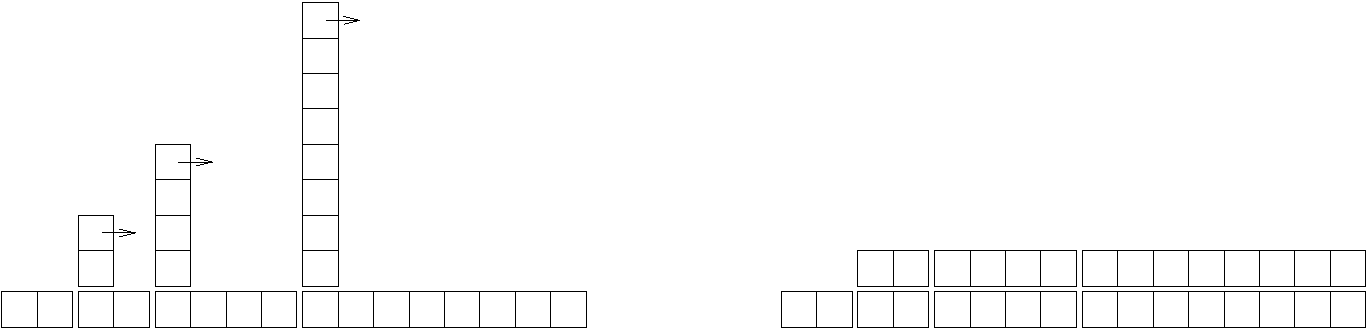
\includegraphics[width=5.5in]{figs/towers.pdf}}
\caption{The cost of a hashtable add.\label{fig.hash}}
\end{figure}

The extra work of rehashing appears as a sequence of increasingly
tall towers with increasing space between them.  Now if you knock
over the towers, spreading the cost of resizing over all
adds, you can see graphically that the total cost after $n$
adds is $2n - 2$.

An important feature of this algorithm is that when we resize the
HashTable it grows geometrically; that is, we multiply the size by a
constant.  If you increase the size
arithmetically---adding a fixed number each time---the average time
per {\tt add} is linear.
\index{geometric resizing}

You can download my implementation of HashMap from
\url{http://thinkpython2.com/code/Map.py}, but remember that there
is no reason to use it; if you want a map, just use a Python dictionary.

\section{Glossary}

\begin{description}

\item[analysis of algorithms:] A way to compare algorithms in terms of
their run time and/or space requirements.
\index{analysis of algorithms}

\item[machine model:] A simplified representation of a computer used
to describe algorithms.
\index{machine model}

\item[worst case:] The input that makes a given algorithm run slowest (or
require the most space.
\index{worst case}

\item[leading term:] In a polynomial, the term with the highest exponent.
\index{leading term}

\item[crossover point:] The problem size where two algorithms require
the same run time or space. 
\index{crossover point}

\item[order of growth:] A set of functions that all grow in a way
considered equivalent for purposes of analysis of algorithms. 
For example, all functions that grow linearly belong to the same
order of growth.
\index{order of growth}

\item[Big-Oh notation:] Notation for representing an order of growth;
for example, $O(n)$ represents the set of functions that grow
linearly. 
\index{Big-Oh notation}

\item[linear:] An algorithm whose run time is proportional to
problem size, at least for large problem sizes.
\index{linear}

\item[quadratic:] An algorithm whose run time is proportional to
$n^2$, where $n$ is a measure of problem size.
\index{quadratic}

\item[search:] The problem of locating an element of a collection
(like a list or dictionary) or determining that it is not present.
\index{search}

\item[hashtable:] A data structure that represents a collection of
key-value pairs and performs search in constant time.
\index{hashtable}

\end{description}


\chapter{The {\tt passdrill} utility}
\label{passdrill}

\index{passdrill}

This is a full listing of the {\tt passdrill} example. Its main goal is to check the Go syntax highlighting.

\lstinputlisting[language=Golang]{passdrill.go}



\printindex

\clearemptydoublepage
%\blankpage
%\blankpage
%\blankpage


\end{document}
